\chapter*{Proposition 41}



\begin{figure*}[ht]
    \begin{center}
    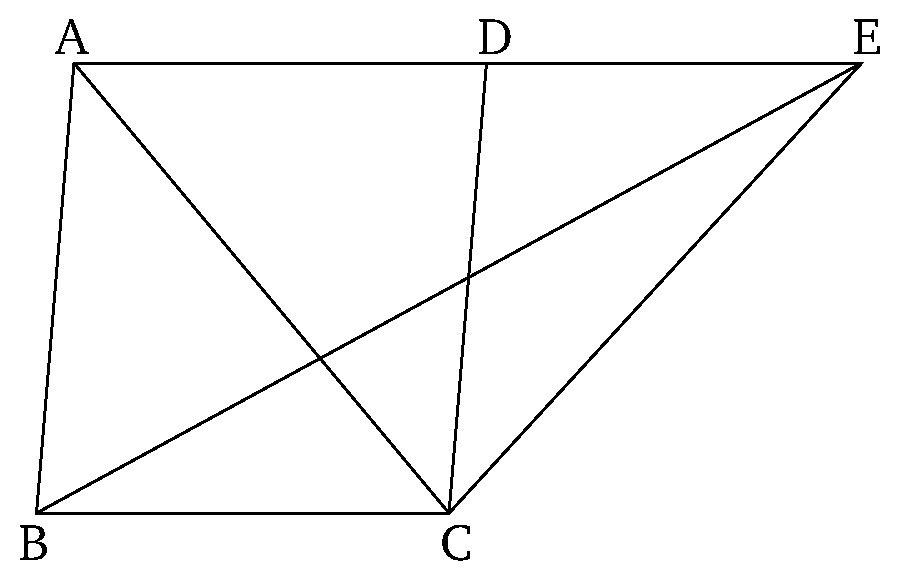
\includegraphics[width=0.5\linewidth]{figures/fig41e.eps}
    \label{fig:prop_41}
    \end{center}
\end{figure*}

If a parallelogram has the same base as a triangle, and is between
the same parallels, then the parallelogram is double (the area) of the triangle.

For let parallelogram $ABCD$ have the same base $BC$ as triangle $EBC$,
and let it be between the same parallels, $BC$ and $AE$. I say that 
parallelogram $ABCD$ is double (the area) of triangle $BEC$.

For let $AC$ have been joined. So triangle $ABC$ is equal to triangle
$EBC$. For it is on the same base, $BC$,  as ($EBC$), and between the same
parallels, $BC$ and $AE$ [Prop.~1.37]. But, parallelogram $ABCD$
is double (the area) of triangle $ABC$. For the diagonal $AC$ cuts
the former in half [Prop.~1.34]. So parallelogram $ABCD$ is also
double (the area) of triangle $EBC$.

Thus, if a parallelogram has the same base as a triangle, and is between
the same parallels, then the parallelogram is double (the area) of the triangle.
(Which is) the very thing it was required to show.


\section*{Commentary}

\begin{proposition}\label{proposition_41}\lean{Elements.Book1.proposition_41}\leanok
    If
\end{proposition}
\begin{proof}
    \uses{proposition_34,proposition_37}\leanok
\end{proof}
